\chapter{Data Analysis}

\section{Efficiencies}
\paragraph{}The high resolution spectrometers are capable of detecting a myriad of particles that track through the detectors. The design of an experimental trigger uses the properties of the individual detectors to capture data of meaningful events. Many accidentals, background, and unwanted events trigger the data acquisition system, and some good electrons are missed by our DAQ. The removal of these unwanted events takes place during analysis via software cuts. Restricting the applicable signal from certain detectors through different cuts allows for the rejection of background particles and prevents contamination in the yield extraction. 

\subsection{Computer and electronic Lifetime}
\paragraph{}The signal from events that fire the DAQ travel through electronics like amplifiers and logic modules on its way to be recorded by the TDCs and ADCs. The processing of these signals require time at each stage. During that time another event will be discarded due to limitations in the hardware. This time when the DAQ system cannot handle another event is known as the dead-time of the system. Lifetime therefor is the percentage of time when an event can be recorded. The lost events need to be account for during the analysis process. The lifetime of the DAQ system for the MARATHON experiment was measured by determining the percentage of events that were recorded relative to the number of events that fired the corresponding trigger. The lifetime for the MARATHON experiment depended on the rate of events. The lifetime during the highest rate kinematic was determine to be 0.947, and climbs to 0.998 for the highest angle setting. Listed in table \ref{LTtable} are the calculated values for lifetime at each kinematic. 

\begin{table}[]
	\textbf{Livetime for each kinematic }\par\medskip
	\begin{tabular}{|l|l|l|l|l|l|l|l|l|l|l|}
		\hline
		Kin      & 1 & 2 & 3 & 4 & 5 & 7 & 9 & 11 & 13 & 15 \\ \hline
		LiveTime & 0.947 & 0.969 & 0.981 & 0.986 & 0.992 & 0.996 & 0.997 & 0.998  & 0.998  & 0.998\\ \hline
	\end{tabular}
	\caption{Livetime during the MARATHON experiment calculated using trigger 2.  }
	\label{LTtable}
\end{table}
  

\subsection{Particle Identification Efficiency}
\paragraph{} One of the largest sources of contamination for the MARATHON experiment are negatively charged pions. These pions are removed through software cuts made in the total signal from the ten cherenkov PMTs(photomultiplier tubes) and the energy deposited into the blocks of both layers of the calorimeter. Electrons can be identified by their behavior in the spectrometer. High-quality electrons will track through the entire detector stack to deposit most of their energy into the total calorimeter system and creating a large amount of light in the cherenkov. Though this knowledge tight cuts can be used to study the efficiency of the particle identification system. Plotting the signal in the cherenkov versus the energy deposited into both layers of the calorimeter allows for visual representation of the sampling cuts made in the efficiency studies, which can be seen in figure \ref{elesample}. 
\begin{equation}\label{effequ}
\begin{split}
GE_{sample} & = \textrm{Known electron sample from tight cut}  \\
GE_{pass} & = \textrm{$GE_{sample}$ and pass indentification cut} \\
Electron_{eff}  & = \frac{ GE_{pass} } { GE_{sample} } 
\end{split}
\end{equation}
\begin{figure}[]
	\centering
	\textbf{Cherenkov sum versus Total Energy deposited }\par\medskip
	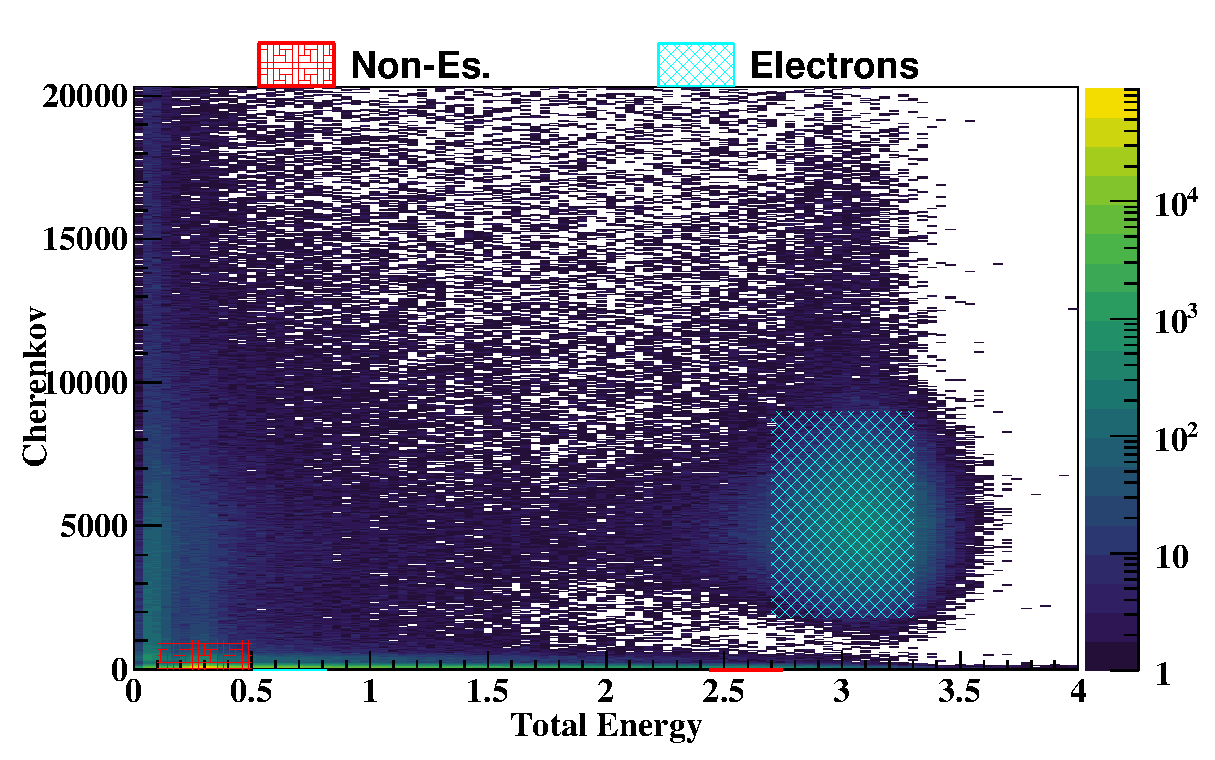
\includegraphics[width=13cm]{PID_2d}
	\caption{Two dimensional plot of the cherenkov sum versus Total Energy deposited, including electron sampling in teal and non-electron sampling in red. }
	\label{elesample}
\end{figure}

\begin{figure}[t]%
	{\centering
		\textbf{Particle ID and efficiency sampling for PID detectors }\par\medskip}
	\centering
	\subfloat[]{\includegraphics[width=0.5\textwidth,height=4.5cm]{Lprl1}\label{samA}}%
	\subfloat[]{\includegraphics[width=0.5\textwidth,height=4.5cm]{Lprl2}\label{samB}}\\
	\subfloat[]{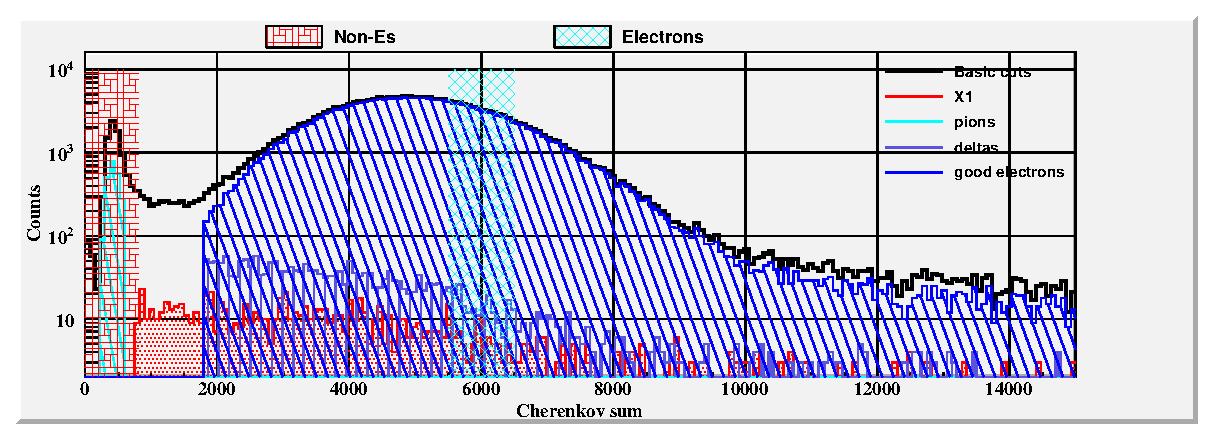
\includegraphics[width=0.95\textwidth,height=3.85cm]{Lcerasum}\label{samC}}%
	\caption{Electrons and other back ground particles identified via cuts in the total calorimeter and the gas cherenkov shown in the individual layers of the calorimeters and the cherenkov. Sampling cuts for Electrons in teal and Non-Electrons in red.}%
	\label{sampling}%
\end{figure}


\paragraph{}The efficiencies of the spectrometer's particle identification(PID) detectors were determined by using the first calorimeter layer, the second calorimeter layer, and the cherenkov to provide samples of good electrons and other particles. The PID efficiency of the individual detectors was determined using equation \ref{effequ}. The good electron sample for calculating the efficiency of the single detector was defined by sampling through the other two detectors. Sampling through the two layers of the calorimeter is shown in figure \ref{samA} for the first layer of the calorimeter and \ref{samB} for the second layer. The cherenkov good electron sample is shown in figure \ref{samC}. The electron sample from the cherenkov is contaminated by delta particles and a combination of unknown particles. These unidentified background particles are known to be relativistic due to the amount of light seen in the cherenkov. However, the events do not deposit enough energy into the calorimeter system to be considered as a good electron that scatter from our target through the detector. Using sampling in one layer of the calorimeter and the cherenkov, these unwanted low energy particles are rejected from sampling for efficiency calculations. The electron selection PID efficiency for the three PID detectors was determine at each kinematic setting to be approximately 98$\%$ . The efficiency was determined to be independent of the kinematic setting. Only small fluctuations were seen during the study, these small changes are due to decrease in statics, and all of the results fall within statical uncertainty of being independent of kinematic setting. The non-electron suppression efficiency was determine as part of this PID efficiency study to ascertain how many back ground particles leak into our sample of good electrons after cuts our made. The suppression efficiency of the cherenkov suffered due to the contamination of the relativistic low energy particles. Combining the two calorimeter detectors with the cherenkov increased the overall suppression efficiency for the spectrometer to 99.9$\%$ over the entire kinematic range of the MARATHON experiment. 

\begin{figure}
	{\centering
		\textbf{PID efficency for each detector for all kinematics. }\par\medskip}
	\centering
	\includegraphics[width=12cm]{PID_allkin_alltgt}
	\caption{The PID efficiency for the cherenkov and both layers of the calorimeter,including the overall total PID efficiency for each of the gas targets at all of the kinematics.}
\end{figure}

\subsection[]{Trigger Efficiency}
\paragraph{} The process of capturing data from the two HRSs begins with the firing of a trigger. The trigger design for MARATHON focused on triggering for electrons and reducing the amount of other particles. Figure \ref{trigger_Setup} describes the design of MARATHON's main trigger and efficiency triggers. MARATHON's main trigger, trigger 2, consist of a $(S_o \& S_2) \& Cer$. Due to inefficiencies of the electronics, logic, and detectors an event can produce a false trigger or a high quality electron may not fire 
the main trigger.

\begin{figure}[]
	\centering
	\textbf{Trigger efficiency for the MARATHON experiment }\par\medskip
	\includegraphics[width=13cm]{Trigger_Eff.eps}
	\caption{Trigger efficiency of trigger 2 for different targets at all kinematics calculated via sampling from trigger 1. }
	\label{trigeff}
\end{figure}

\paragraph{} A low threshold in the cherenkov allows for an inclusive trigger limiting the overall number of quality electrons missed, but allows for a large quantity of false triggers. Software PID cuts prevent the contamination of false positives from trigger inefficiencies. The tight PID software cuts removes the false positive inefficiency from the trigger design and is then considered in the PID efficiencies. The trigger inefficiency caused by missed high quality electrons was then calculated by sampling the high quality electrons in trigger 1, $(S_o \& S_2)$. This ties the efficiency of trigger 2 with the performance of the scintillators. The efficiency of the two scintillating planes in conjunction is calculated by using sampling in trigger 3, $(S_o | S_2) \& Cer$ with strict PID cuts in both layers of the calorimeters and requiring a hit in the cherenkov. The two scintillator planes in conjunction have an efficiency greater than $99.7 \% $ for all kinematics. Combining the trigger efficiency of the main trigger shown in figure \ref{trigeff} with the performance of the scintillators give an over all efficiency for the trigger of the MARATHON experiment of greater then $99.6\%$.

\subsection[]{Tracking Efficiency}
\begin{figure}[]
	\centering
	\textbf{Tracking efficiency for the MARATHON experiment }\par\medskip
	\includegraphics[width=11cm]{Tracking_Eff_allkin.eps}
	\caption{Tracking efficiency of the VDCs for different targets at all kinematics. }
	\label{trackeff}
\end{figure}
\paragraph{}Particles that travel through our detector could originated from sources wanted or unwanted. In order to control the source of the scatter electrons, we use a particle's track to identify its source. The signals received via the VDC is used to produce a particles track from the target to end of the spectrometer. The largest source of inefficiency for the VDCs are incorrectly identified tracks. High quality electrons that transverse the spectrometer should only have one good track, calculated via the tracking package in the analysis software. The capability of the VDCs to determine a good electron event's one good track is know as the one track efficiency for the VDCs. Quantitatively the one track efficiency ($\epsilon_{VDC}$) can be obtained via:
\begin{equation}
\epsilon_{VDC} \equiv \frac{N_{1 track} }{N_{0 \& multitrack}}
\end{equation}
Where the number of good electron events that have one good track is defined as $N_{1 track}$, and $N_{0 \& multitrack}$ are the good electron events that have not been assigned a good track or have more then one good track associated with that event. The good electron selection is made via PID cuts in the calorimeter and cherenkov, and cuts in the ADC and TDC of the scintillators. Direct cuts in the signal of the scintillators where made to include the nominal acceptance cuts, which our produced through tracking software. The tracking efficiency of HRSs during the MARATHON experiment is shown in figure \ref{trackeff} for the three gas targets during all kinematic ranges. The efficiency of the VDCs is not relative to the angle of the spectrometer. So the uniform tracking efficiency across all kinematics is expected and helps eliminate any concerns of the performance of the VDCs during the experiment. 

\section{Background Subtraction}
\paragraph{} The purpose of this analysis is to study the DIS cross sections of deuterium, helium-3, and tritium. The sample of scattered events used to determine the cross section of a given nuclear then needs to be cleaned of any contamination produced from other targets and processes. The electrons detected by the spectrometers can be electrons that scatted from our chosen target, scattered from a source other then our target, or produced through process other than DIS scattering. The two sources of contamination for the MARATHON experiment are events scattered from the aluminum end caps of the target cell and pair produced electrons via photon interaction. 
\subsection{End Caps}
\paragraph{} The target cells used during the MARATHON experiment are shown in figure \ref{HATT}. The cells are filled with gaseous version of the chosen nuclear target. 
\subsection{Pair Produced Electrons}





